\chapter{Fundamentação}\label{ch:Fundamentacao}

A fundamentação teórica é um elemento crucial para a compreensão dos fundamentos teóricos que dão base aos conceitos que permeiam o objeto de estudo em uma determinada pesquisa. O capítulo de fundamentação surge então para munir o pesquisador dos conhecimentos necessários para o andamento e a conclusão de sua pesquisa. Ao mesmo tempo, a fundamentação auxilia outros pesquisadores na identificação das bases do conhecimento teórico que guiaram determinado estudo. 

O corrente estudo tem como cerne a validação de um programa educacional para a prevenção da violência sexual infantil baseado na dinâmica de jogos. Deste modo, a \autoref{sec:JogosSerios} traz fundamentação sobre os jogos na educação. A \autoref{sec:Engenharia} traz alguns conceitos sobre o desenvolvimento de jogos. A \autoref{sec:Avaliativos} discute sobre modelos voltados para a avaliação de programas educacionais na temática de prevenção a violência sexual infantil.

%-------------------------------------------------------------------------------------------------------------------
\vspace{1.0 cm}
\section{Jogos Sérios}\label{sec:JogosSerios}

Jogos com propósitos educacionais existem a várias décadas. Ao longo dos anos, tais jogos tiveram várias denominações e definições. Dentre as denominações, a que melhor define o contexto desta pesquisa é o termo \ac{JS} (em inglês: \textit{Serious Game}), usado pela primeira vez na história em \citeyear{clark1970serious} \cite{djaouti12011origins}. Desde \citeyear{clark1970serious}, o termo passou por inúmeras revisões até alcançar sua definição atual, a qual compreende como \ac{JS}: todos os jogos projetados para uma finalidade principal que não a pura diversão \cite{michael2005serious, laamarti2014overview, carvalho2015aprendizagem}.

A definição atual de \ac{JS} permite identificar que os jogos classificados como sérios antecedem a própria origem do termo. Isso pois, a história conta que antes da década de 70, alguns jogos já eram utilizados para outros propósitos além do entretenimento \cite{wilkinson2015brief}. Salienta-se, no entanto, que o termo não encontra-se verdadeiramente consolidado na literatura científica da área, existindo inclusive várias definições e termos correlatos \cite{pourabdollahian2012serious}.

Para definir melhor o termo \ac{JS} que fundamentará e guiará o andamento do presente estudo, buscou-se separar o conceito e interpretar individualmente as palavras que o compõem. O termo \textbf{Jogo} demarca o conjunto de atividades regidas por uma estrutura de regras focadas na diversão e no entretenimento \cite{kishimoto1994jogo}. Já o termo \textbf{Sério} define um propósito prático a este conjunto de atividades, geralmente sendo pedagógico, comportamental ou motor \cite{schroeder2017wobu, baptista2017jogos}. %(com os Exergames = Jogos Ativos). 
A Figura \ref{fig:JS}, ilustra de forma resumida os conceitos que fundamentam a definição de \ac{JS} do atual trabalho. 

\pagebreak

\begin{figure}[htb]

	\caption{\label{fig:JS}Infrográfico da terminologia Jogo Sério.}\vspace{-0.1cm}
  \hspace{-0.9cm}
  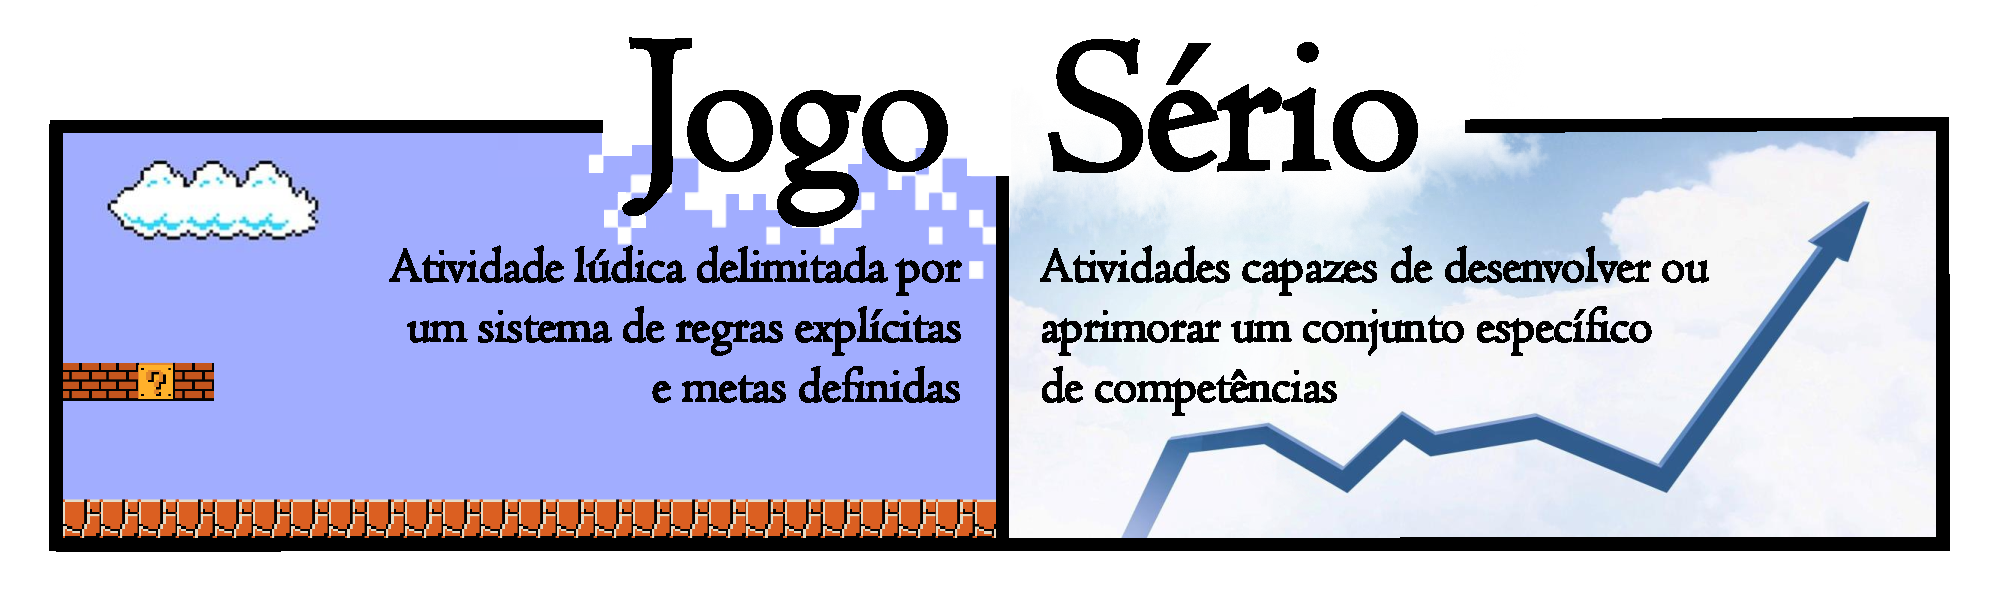
\includegraphics[width=1.1\linewidth]{./Visuais/JogoSerio.pdf}\vspace{-0.1cm}
  \legend{Fonte: Elaborada pelo autor (2020).}

\end{figure}

A Figura \ref{fig:JS} define separadamente a palavra \textbf{Jogo} e \textbf{Sério}. A união das definições dá o conceito de \ac{JS} mais comum encontrado em pesquisas na área \cite{michael2005serious}. Enfatiza-se que para uma atividade se configurar como \textbf{Jogo}, basta obedecer a um conjunto de regras e objetivos. Um jogo nessa definição não precisa de quaisquer outros artefatos para se configurar como tal, podendo ainda, ocorrer individualmente ou coletivamente. Para um jogo abranger o caráter \textbf{Sério} é necessário que o mesmo trabalhe em algum nível as habilidades físicas, comportamentais, ou intelectuais de seus jogadores. 

O aprimoramento ou desenvolvimento de habilidades físicas normalmente é associado aos \textbf{Jogos Ativos} (em inglês: \textit{Exergames}) \cite{araujo2017exergames, schroeder2017wobu}. Já o aprimoramento ou desenvolvimento de habilidades intelectuais é geralmente relacionado aos \textbf{Jogos Educativos}. Pode-se dizer então que a classe de \ac{JS} é uma generalização das áreas de \textbf{Jogos Ativos} e \textbf{Jogos Educativos}. Salienta-se, no entanto, que para um jogo ser classificado como \textbf{Sério}, não se faz necessário que o jogo compreenda ambas as áreas. Todavia, na definição mais aceita, um \ac{JS} deve abranger a área dos \textbf{Jogos Digitais} \cite{laamarti2014overview}.

Os \textbf{Jogos Digitais} são todo o conjunto de jogos, os quais são jogáveis apenas por intermédio de mídias digitais \cite{lucchese2009conceituaccao}. Os jogos digitais, englobam a definição clássica de \textbf{Jogo}, necessitando também de um conjunto de regras e objetivos, porém acrescidos de um motor de jogo e uma interface interativa \cite{battaiola2000jogos}. Enquanto o motor de jogo fica responsável por controlar o conjunto de regras que rege o jogo. A interface interativa se encarrega de converter o jogo em si para sinais visuais e sonoros compreensíveis ao jogador.

Os \textbf{Jogos Digitais}  possuem um sistema de regras mais rígido em relação aos jogos clássicos, devido ao contexto computacional do motor de jogo. O mesmo contexto computacional também é responsável por trazer maior segurança aos \textbf{Jogos Digitais}  em relação aos clássicos, uma vez que a interface interativa é capaz de construir um ambiente lúdico inteiramente virtual, no qual os jogadores possam passar por situações de perigo sem que isso reflita em vias de fato em riscos aos jogadores \cite{lucchese2009conceituaccao}.

Os \acp{JS} assumem um importante papel no aprimoramento das habilidades de seus jogadores à medida que proporcionam um ambiente seguro de interação. Ou seja, \acp{JS} são \textbf{Jogos Digitais}, porém projetados de modo que seus jogadores desenvolvam novas competências e/ou conhecimentos, ou reforcem capacidades existentes \cite{boller2017play}. O contexto digital de tais jogos ainda permite um sistema totalmente livre de julgamentos \cite{unesco2018international}. A depender da dinâmica do jogo, é possível que o jogador interaja com o ambiente virtual do jogo sem que seus erros tenham forte impacto no seu contexto social. Ou seja, o ambiente virtual de um jogo permite aos jogadores um espaço sem pressão social, no qual podem jogar o jogo sem se sentirem acanhados ou tímidos.

Os \acp{JS} proporcionam um sistema de aprendizagem interativa. A aprendizagem interativa é um processo didático de ensino mais atrativo aos \acfp{ND}. Os \acp{ND} apresentam maior preferência por abordagens interativas baseadas em processos de tentativa e erro \cite{pescador2010tecnologias}. Além disso, os \ac{ND} já nascem imersos no mundo digital, o que torna para eles, o processo de iteração com artefatos digitais, um processo mais natural e orgânico, em comparação a iteração entre tais artefatos e os \acfp{ID}.

Os \acp{JS} manifestam-se como um facilitador do processo de aprendizado dos \acp{ND}. A abordagem de \ac{JS} no ambiente escolar pode trazer benefícios ao processo de ensino-aprendizagem, proporcionando um sistema motivador para o desenvolvimento de habilidades cognitivas, além de garantir um sistema de aprendizado por descobertas \cite{carvalho2017move4math}. Um ambiente de aprendizado por descoberta desenvolve o pensamento abstrato dos jogadores, obrigando-os a solucionar problemas inéditos. A solução de problemas inédito é alcançada través de deduções realizadas em comparação a problemas similares apresentados previamente aos jogadores. É crucial que a solução de problemas por meio de \ac{JS} assuma um caráter lúdico que divirta os jogadores na mesma medida que os eduque, para garantir assim, uma maior retenção do conteúdo ensinado \cite{tarouco2004jogos}. 

O presente estudo desenvolve um \ac{JS} objetivado a compor um programa educacional para a prevenção da violência sexual infantil. A compreensão dos fundamentos que definem um \ac{JS} é indispensável para a progressão e conclusão deste trabalho. Buscando trazer maior alcance ao jogo desenvolvido, o jogo em si está exportado para navegadores. Tal característica não fere a definição de \ac{JS}, uma vez que a definição não especifica os meios eletrônicos de acesso ao jogo. Sendo assim, um \ac{JS} para navegadores, permite que um determinando jogo possa ser jogado em qualquer dispositivo com acesso a rede, sem quais restrições mais severas de memória ou processamento. 

O presente trabalho baseia-se nos conceitos pesquisados e nas definições referenciadas nessa seção para fundamentar o \ac{JS} desenvolvido. Não cabe a apresente seção a descrição das temáticas e dos conceitos abordados no jogo. Nesse sentido, salienta-se que a estrutura lúdica e pedagógica do jogo são conceitos abordados por essa dissertação apenas no Capítulo \ref{ch:Desenvolvimento}.

%-------------------------------------------------------------------------------------------------------------------

\section{Metodologia de Desenvolvimento de Jogos}\label{sec:Engenharia}

O mercado de jogos movimenta bilhões de reais todos os anos ao redor do mundo \cite{fortim2020games}. A indústria de desenvolvimento de jogos acompanha essa cifra trazendo cada vez mais pessoas capacitadas para a produção e desenvolvimento de jogos. Em alguns casos o processo de desenvolvimento de um jogo pode envolver milhares de pessoas e levar anos até ser finalizado. Em contrapartida há ainda os jogos de caráter mais independente (\textit{indie game}) que acabam por serems jogos mais modestos em termos de desenvolvimento, se limitando a equipes pequenas, podendo ser produzidos em pouco tempo, ou não. Essa discrepância entre os jogos resulta em uma quantidade variada de metodologias voltadas para o desenvolvimento de jogos.

As metodologias para o desenvolvimento de jogos variam a depender de uma série de fatores. Entretanto, três questões principais são levadas em consideração no momento da escolha por uma metodologia: quantidade de envolvidos no projeto, prazo da entrega e recursos necessários. No mais, após o prazo de entrega, um jogo ainda pode passar por um processo de manutenção trazendo otimizações e customizações ao jogo no decorrer de vários anos. Embora muitos estudos tenham sido publicados sobre o desenvolvimento de jogos para a área da educação, existem poucas metodologias reconhecidas nesta área \cite{aslan2015gamed}. Somado a isso, a literatura informa que o desenvolvimento individual de um produto não precisa necessariamente seguir uma metodologia \cite{valente2021engenharia}. Todavia, no caso do desenvolvimento de jogos educacionais digitais a utilização de uma metodologia é capaz de fornecer uma abordagem estruturada centrada na qualidade do jogo garantindo o cumprimento de objetivos de aprendizagem exigentes no jogo. Sendo assim, o \ac{JS} escolhido pelo presente trabalho para compor um programa de prevenção a violência sexual infantil tem seu desenvolvimento baseado em uma metodologia reconhecida voltada para o desenvolvimento de jogos educativos digitais denominada de \ac{GAMED} \cite{aslan2016digital}. 

A metodologia \ac{GAMED} é uma metodologia voltada para o desenvolvimento de jogos educacionais digitais, podendo ser aplicada tanto para grandes ou pequenos projetos. O \ac{GAMED} apresenta alta qualidade, baixo risco de falhas e alta probabilidade de que o jogo seja concluído dentro do orçamento e prazos estabelecidos \cite{aslan2015gamed}. Além disso, o \ac{GAMED} fornece uma abordagem modular estruturada para superar a complexidade do desenvolvimento e orienta os desenvolvedores durante todo o ciclo de desenvolvimento do jogo.

O \ac{GAMED} é uma metodologia que se incrementa a cada ciclo de desenvolvimento. Ao final de cada ciclo há a entrega de um jogo operacional, por tal razão o \ac{GAMED} pode ser classificado como um método ágil de desenvolvimento. O \ac{GAMED} é constituído por quatro fases principais: Fase de Projeto, Fase de Projeto de \textit{Software}, Fase de Desenvolvimento/Publicação e Fase de Realimentação. As fases são subdivididas em etapas, cada etapa consiste de um processo. A \autoref{fig:GAMED} apresenta um esquema com os principais elementos requeridos no \ac{GAMED}. 

\pagebreak

\begin{figure}[!ht]

	\caption{\label{fig:GAMED}Ciclo de Desenvolvimento de Jogos da Metodologia GAMED.}
  \begin{center}%\vspace{-0.3cm}
    \frame{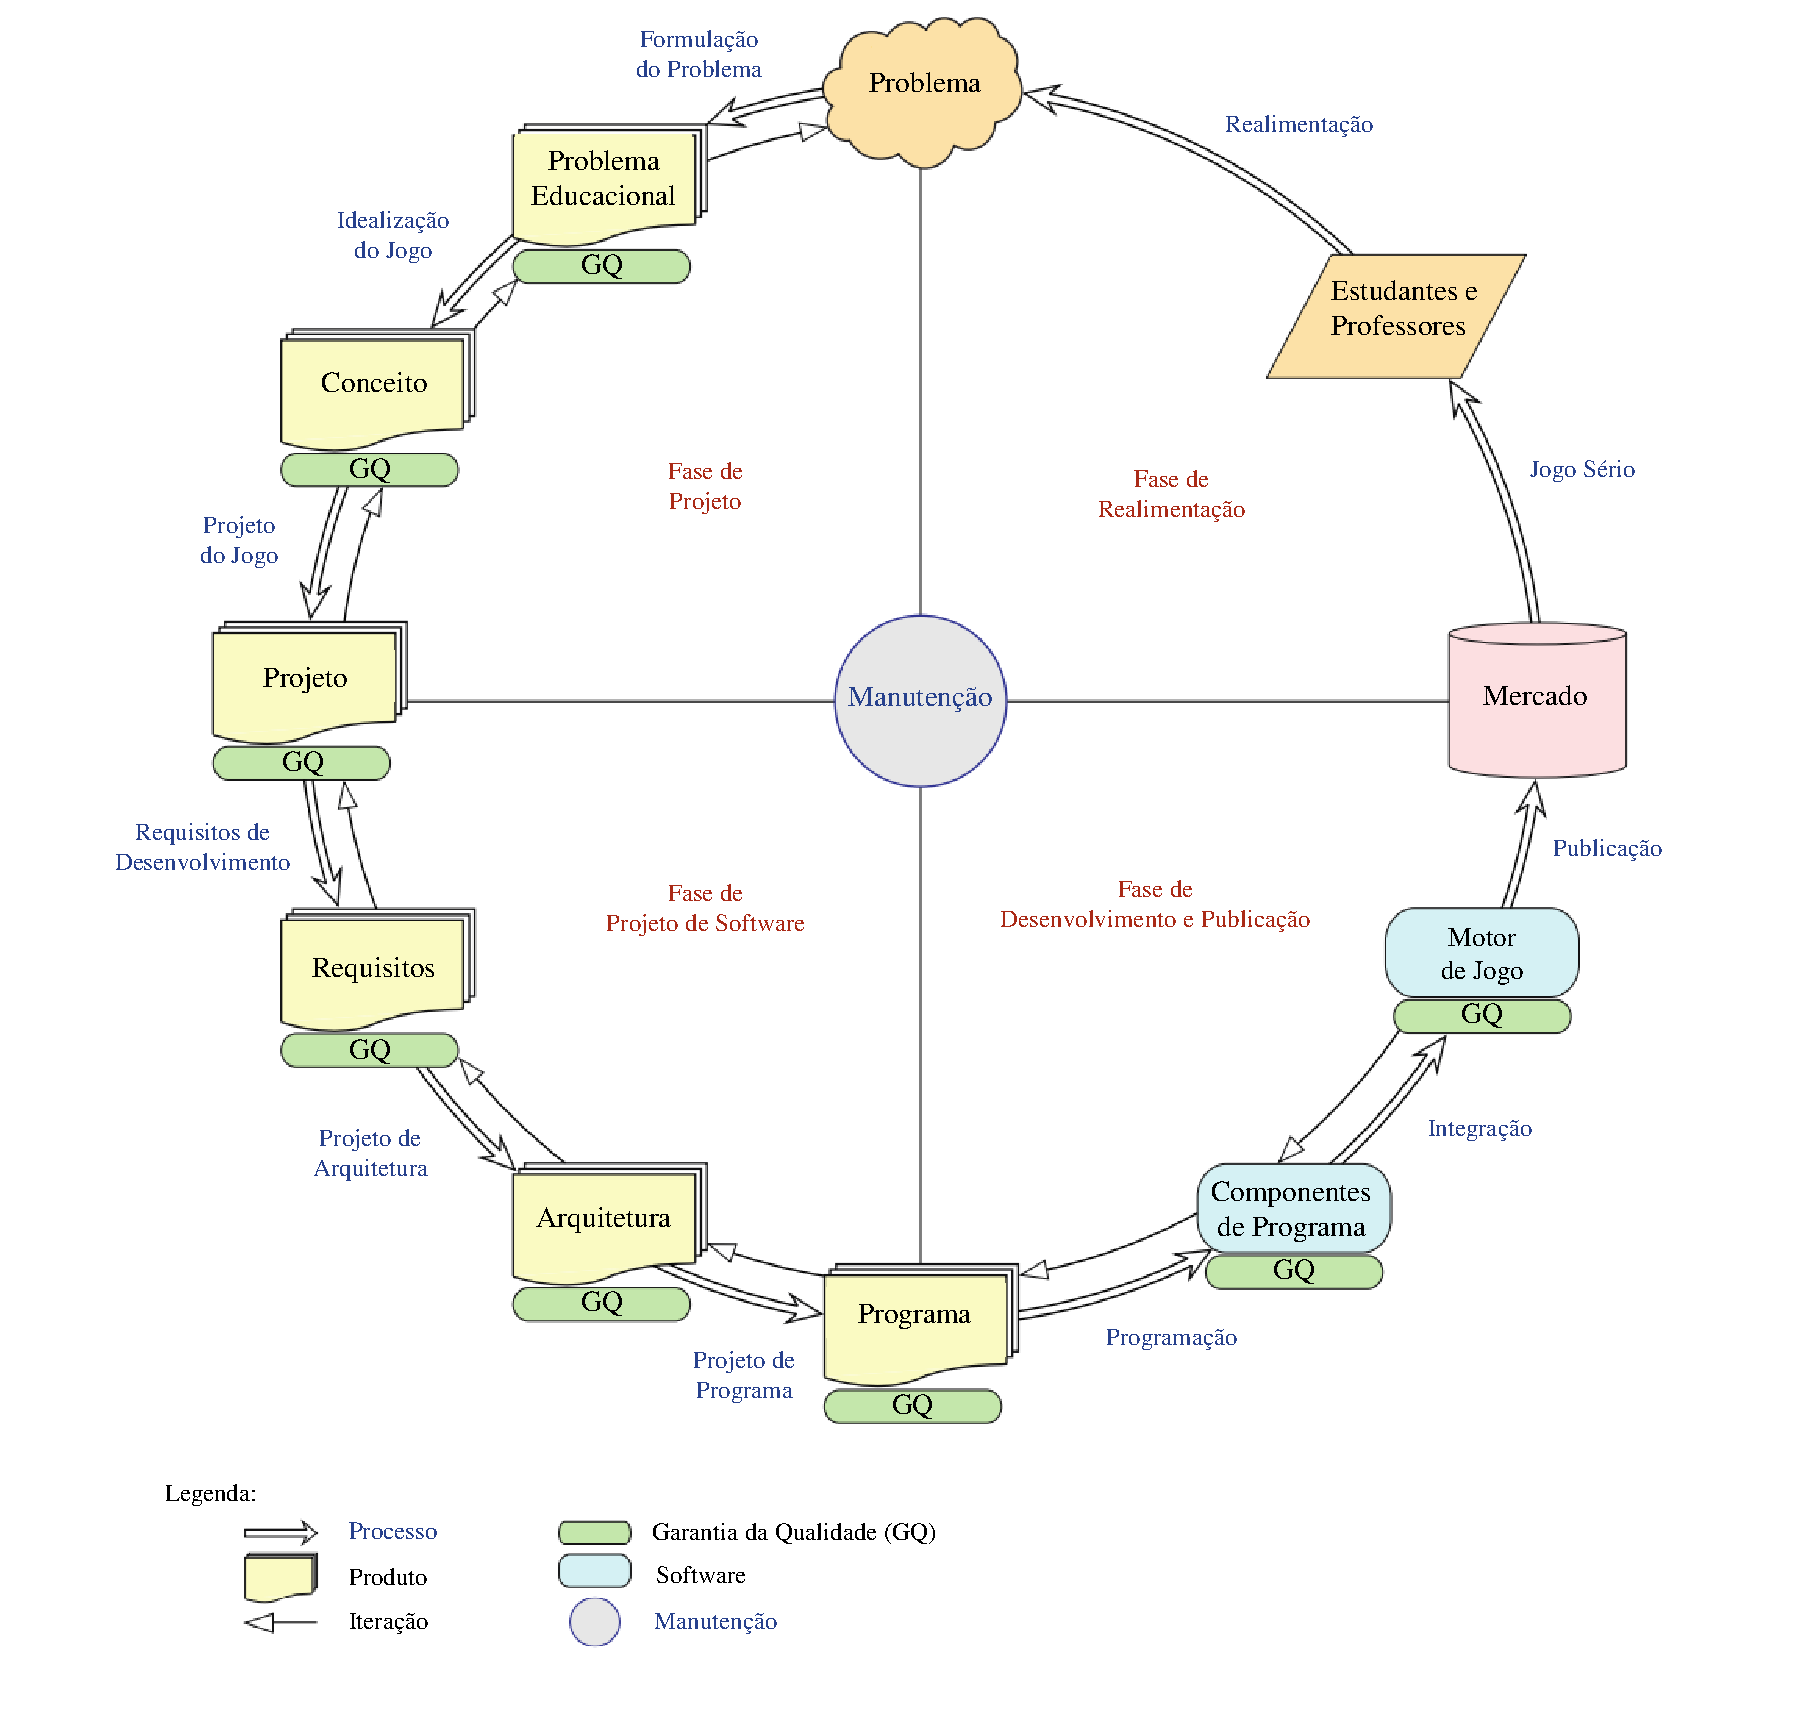
\includegraphics[width=\linewidth]{./Visuais/GAMED.pdf}}
	\end{center}%\vspace{-0.5cm}
  \legend{Fonte: adaptado de \citeonline[p. 23]{aslan2016digital}.}

\end{figure}


O ciclo da \autoref{fig:GAMED} apresenta os processos em uma forma lógica solicitante começando de um \textbf{Problema} inicial. A partir de então o ciclo se inicia na Fase de Projeto, passando pelo Projeto de \textit{Software}, pela Fase de Desenvolvimento e pela Fase de Realimentação. Ao término da última fase o ciclo se inicia novamente sendo um processo de manutenção contínuo do jogo. Cabe salientar que embora as setas mostrem um progresso sequencial, o ciclo de desenvolvimento de um jogo não precisa ser interpretado como estritamente sequencial. A representação sequencial usada na \autoref{fig:GAMED} se destina a mostrar apenas a direção do fluxo de trabalho ao longo do ciclo de desenvolvimento. 

\pagebreak

A metodologia \ac{GAMED} é iterativa tanto em sentido horário, quando em sentido anti-horário. No caso, as setas reversas almejam sanar um problema relativamente comum na área de desenvolvimento de jogos (\textit{e.g.} um determinado processo pode apontar falhas no processo anterior; para arrumar a falha é recomendado retornar ao processo anterior ao invés de esperar que o ciclo se complete por inteiro). A alternância entre os processos acontece após atingir um patamar aceitável de confiança na qualidade do jogo, por tal razão cada processo passa por uma etapa de \textbf{\ac{GQ}}. A qualidade só é atingida após um grupo qualificado confirmar que os seguintes conceitos estão devidamente empregados no jogo desenvolvido: Aceitabilidade, Desafio, Clareza, Eficácia, Engajamento, Diversão, Interatividade, Flexibilidade/Escalabilidade, Ludificação, Simplicidade, Aprendizagem e Usabilidade. 

A primeira fase do \ac{GAMED} (\textbf{Fase de Projeto}) estabelece a definição de um problema no domínio educacional para ser abordado por meio da dinâmica de jogos. O atual trabalho se objetiva a fortalecer as estratégias de enfretamento ao problema da violência sexual infantil. Por tal razão, foi realizada uma formulação do problema, identificando suas causas e consequências, além da criação conceitual do jogo. Na segunda fase do \ac{GAMED} (\textbf{Fase de Projeto de Software}); referente ao jogo produzido por este trabalho; foram catalogados os requisitos necessários para o desenvolvimento do jogo, além da escolha da arquitetura a ser utilizada. Um documento de requisitos é produzido nesta etapa. A terceira fase do \ac{GAMED} (\textbf{Fase de Desenvolvimento/Publicação}), remete especificamente ao processo de criação e desenvolvimento do jogo. O jogo deve ser produzido nesta etapa de modo a sempre disponibilizar ao final uma versão jogável. A quarta fase do \ac{GAMED} (\textbf{Fase de Realimentação}), busca apresentar um jogo brevemente finalizado a estudantes ou professores. O intuito é identificar falhas ou eventuais melhorias que podem vir a serem relatadas. Nesta etapa o jogo pode ser apresentado a outros profissionais devidamente capacitados que não precisam necessariamente contemplar o público-alvo do jogo.

O \ac{GAMED} fornece um plano detalhado para o gerenciamento de projetos complexos de desenvolvimento de jogos. Sua estrutura modularizada de desenvolvimento em fases e processos facilita o desenvolvimento de jogos educacionais digitais. O \ac{GAMED} ainda é flexível se adaptando as necessidades da equipe de desenvolvimento \cite{aslan2016digital}. Como o desenvolvimento do \ac{JS} deste trabalho envolveu essencialmente uma pessoa (o próprio pesquisador) algumas etapas do \ac{GAMED} foram supridas a fim de agilizar o processo de desenvolvimento, porém sem perder sua essência primordial. 

A compreensão dos fundamentos acerca o desenvolvimento de jogos educacionais digitais é indispensável para a progressão e conclusão deste trabalho. O presente trabalho baseia-se nos conceitos pesquisados e nas definições referenciadas nessa seção para fundamentar o processo de desenvolvimento.

%-------------------------------------------------------------------------------------------------------------------

\section{Metodologia Avaliativa}\label{sec:Avaliativos}

A avaliação de jogos educativos busca medir o seu nível de sucesso no âmbito educacional. Em outras palavras, metodologias avaliativas associadas a jogos buscam identificar se um determinado jogo é capaz de alcançar com os objetivos pré-estabelecidos. A metodologia utilizada pela presente pesquisa para constatar a eficácia de um jogo como solução educacional para prevenção da violência sexual infantil é composta por 7 (sete) procedimentos. Cada procedimento é abordado separadamente em uma subseção específica. Desta forma, a \autoref{subsec:legais} aborda sobre as considerações legais da corrente pesquisa, a \autoref{subsec:segmentacao} fala sobre o processo de segmentação da amostra, a \autoref{subsec:preteste} menciona sobre a etapa de pré-teste, a \autoref{subsec:teste} fala sobre a etapa de teste, a \autoref{subsec:posteste} discorre sobre a etapa de pós-teste, a \autoref{subsec:grupo} menciona sobre o processo de apreciação, a \autoref{subsec:documentacao} trata da etapa de documentação dos achados e a \autoref{subsec:CF} dá as conclusões da presente seção. A ordem dos procedimentos apresentados, corresponde a ordem de andamento deles na presente pesquisa. 

\subsection{Considerações Legais}\label{subsec:legais}

As considerações legais englobam toda a documentação jurídica necessária para a condução de uma determinada pesquisa. Quaisquer estudos que envolvam seres humanos como instrumento de pesquisa devem ter seus procedimentos devidamente analisados. Além disso, o envolvimento de instituições ou indivíduos deve ser judicialmente formalizado. A presente pesquisa é projetada de modo a conduzir parte de seus procedimentos em escolas da rede pública do ensino fundamental. O documento que formaliza a parceria entre essa pesquisa e escolas da rede pública é a Declaração de Ciência e Concordância das Instituições Envolvidas (\autoref{chap:DIE}). 

As parcerias firmadas pela corrente pesquisa, com escolas da rede pública, ocorrerem em comum acordo com os representantes legais das instituições de ensino envolvidas e com a \ac{SED} do município de Joinville do estado de \ac{SC}. %Salienta-se que são firmadas parcerias apenas com as escolas com corpo docente disponível para a execução dos procedimentos desta pesquisa. Isso pois, os pesquisadores são incapazes de executar os procedimentos desta pesquisa nas escolas devido há restrições legais\footnote{Portaria Conjunta SES/SED Nº 476. Art. 18 Nos estabelecimentos de ensino que ofertam o Ensino Fundamental anos iniciais, os Planos de Contingência, além das medidas sanitárias gerais determinadas nos incisos dos Art. 10 a 17 desta portaria, deverão organizar as medidas específicas de prevenção e controle relacionadas ao ensino fundamental anos iniciais, a fim de combater e mitigar o contágio da COVID-19: VI. Não é permitida a implementação dos programas e projetos intersetoriais e atividades, que são desenvolvidos por profissionais que não fazem parte do corpo docente da unidade escolar.}.
Salienta-se que o cronograma do atual estudo é devidamente deliberado com as escolas parceiras de modo a conduzir a pesquisa sem grandes prejuízos a agenda escolar das crianças. Isso pois, todos os procedimentos envolvendo a participação de crianças no presente estudo ocorre em ambiente escolar e em horário escolar (visando agilizar o andamento e a conclusão da pesquisa). Uma vez delimitadas as datas, o envolvimento das crianças no presente estudo se inicia. 

A participação de quaisquer indivíduos em pesquisa científica deve ser firmada por meio de um documento legal. A utilização de crianças como instrumento de estudo torna necessário que as crianças atestem sua anuência em participar da pesquisa. Além disso, também é preciso a autorização formal de seus representantes legais. O documento que firma a participação de crianças na corrente pesquisa é o Termo de Assentimento (\autoref{chap:TA}). Já a autorização formal dos representantes legais das crianças é firmada pelo Termo de Consentimento Livre e Esclarecido (\autoref{chap:TCLE}). Ambos os documentos devem estar devidamente assinados para que seja válida a participação de uma determinada criança no presente estudo. %Todavia, o mesmo não se faz válido para o Termo de Consentimento para Fotografias, Vídeos e Gravações (\autoref{chap:TCF}).

%O registro de informações visuais ou sonoras ajudam as pesquisas científicas que dependem da coleta deste tipo de informação. Todavia, as pesquisas que independem destes registros (como essa pesquisa), os  requisitam para trazer maior transparência e esclarecimento sobre o andamento do estudo e dos experimentos. No entanto, para que a coleta de tais informações seja feita, é preciso a autorização legal de um determinado indivíduo ou de seu representante legal. 

%A corrente pesquisa formaliza o registro de informações visuais ou sonoras no Termo de Consentimento para Fotografias (\autoref{chap:TCF}). O termo em questão não precisa estar assinado para que um determinado indivíduo participe do estudo, justamente por essa não ser uma informação necessário para se alcançar os achados teorizados. 

%http://www1.udesc.br/arquivos/id_submenu/677/resolucao_466_12_cns__ms.pdf = 5 anos





%Os acordos de participação da corrente pesquisa são firmados inteiramente em ambiente escolar. A corrente pesquisa é apresentada ao representante legal da instituição de ensino, o qual deve assinar o documento de Declaração das Instituições Envolvidas. O recurtamento das crianças ocorrerá via a própria escola da criança. Inicialmente será devidamente requisitada a anuência das crianças em participarem da pesquisa por meio do Termo de Assentimento (\autoref{chap:TA}). Para as crianças que concordarem, serão entregues os demais termos para serem apresentados aos seus pais ou responsáveis. Uma das vias de cada termo ficará em posse dos responsáveis pela criança, enquanto a outra deverá ser apresentada na escola e entregue a um dos pesquisadores. Em síntese, a coleta das autorizações será realiza em ambiente escolar por parte dos pesquisadores e em ambiente domiciliar por parte das crianças. No ambiente escolar, a pesquisa e os pesquisadores serão apresentados a uma turma escolar (selecionada para a pesquisa e fornecida pela escola). Será lido então para toda turma Termo de Assentimento da pesquisa. Após a leitura do termo será questionado a turma sobre as crianças interessadas em participar da pesquisa. Aos interessados será entregue o Termo de Assentimento impresso, conjuntamente com os termos: Termo de Consentimento Livre e Esclarecido (\autoref{chap:TCLE}); Termo de Consentimento para Fotografias (\autoref{chap:TCF}). Será requisitado que todos os termos sejam apresentados aos devidos responsáveis legais de cada crianças e assinados. Uma das vias (assinada) deverá ser levada a escola para ser colhida por um dos pesquisadores. Só participarão da pesquisa as crianças que comprovarem autorização dos pais. Visando garantir a integridade das assinaturas e fugir de falsificações cada assinatura será comparada ao documento de matrícula escolar assinado na escola presencialmente pelos pais de cada criança. Salienta-se que a não assinatura dos Termo de Consentimento para Fotografias (\autoref{chap:TCF}) não invalida a participação do menor na pesquisa em questão. Todos os procedimentos legais ocorerrão presencialmente (podendo ser por um dos pesquisadores responsáveis ou por outro responsável optado pela escola). A aplicação da pesquisa de modo presencialmente permite um acompanhamento mais zeloso as crianças, garantido a fiscalização e o monitoramento dos participantes a fim de evitar ao máximo quaisquer danos. Com o término da coleta de documentação legal (prevista para ser concluida em até um mês), a presente pesquisa é capaz de prosseguir para os demais procedimentos.


\subsection{Segmentação}\label{subsec:segmentacao}

Em pesquisa científica, o processo de segmentação está associado, em grande parte, ao isolamento de variáveis. Academicamente, almeja-se isolar variáveis para se compreender melhor os resultados de uma determinada pesquisa. No caso das pesquisas envolvendo seres humanos, o processo de segmentação, normalmente diz respeito a segregação de uma amostra de indivíduos. Para essa pesquisa, o processo de segmentação se deu com base nas turmas escolares das crianças de forma totalmente aleatória. Ou seja, as crianças válidas em participar da presente pesquisa são separadas em dois grupos distintos com base em suas turmas, onde crianças da mesma turma, acabam por pertencer ao mesmo grupo. Os dois grupos que definem o presente estudo são: grupo controle e grupo experimental. 

O grupo controle representa o grupo de indivíduos que não são submetidos a um objeto estudado, servindo como uma variável controle. Já o grupo experimental é o grupo de indivíduos que são submetidos a um objeto estudado. No caso da atual pesquisa o objeto estudado é um jogo educacional para prevenção da violência sexual infantil. Por se tratar de um processo aleatório, é impossível que um determinado indivíduo saiba a qual grupo pertencerá, antes que a etapa de segmentação esteja concluída. A conclusão da presente etapa inicia a etapa de pré-teste. 

%discorrer sobre a separação em grupos da amostra. Em pesquisas experimentais o processo de segementação de uma amostra de indivíduos deve obedecer uma distribuição aleatória. Para essa pesquisa a divisão entre os grupos controle e experimental ocorrerá em turmas escolares (visando agilizar o processo). Isso pois, acredita-se que as turmas de uma escola já são montadas de forma aleatória. Salienta-se que no corrente momento não se sabe da quantidade de crianças que participarão da pesquisa, por tal razão não se sabe quantos grupos controle e experimental existirão, devendo haver no mínimo um grupo de cada com 30 crianças ao menos para essa pesquisa ser encontradas nos requisitos mínimos do rigor científico.

%Nos termos nos quais as assinaturas foram requisitadas (\autoref{chap:TCLE}, \autoref{chap:TA}) não constam o grupo determinado que a criança poderá cair, no entando, todos os procedimentos tomados com cada grupo são descritos. A divisão não ocorrerá de forma presencial. O tempo previsão para essa etapa é de um dia, ao término dessa etapa a presente pesquisa pode adentrar na etapa de pré-teste. 

\subsection{Pré-teste}\label{subsec:preteste}

Na academia científica, a etapa de pré-teste é utilizada normalmente com o intuito de se mensurar uma variável ou um conjunto de variáveis. O objetivo da etapa de pré-teste é justamente coletar informações antes que um determinado experimento ocorra, permitindo assim, uma comparação mais clara, entre os resultados alcançados antes de um teste e os resultados alcançados depois deste mesmo teste. Na área da avaliação cognitiva, a coleta de informações tende a ser realizada por meio de um instrumento avaliativo. No caso, a presente pesquisa tem como foco medir os níveis de conhecimento sobre a prevenção da violência sexual. O modelo avaliativo, mais presente na literatura pesquisada, para se medir os níveis de conhecimento sobre a prevenção da violência sexual é o \ac{CKAQ}.

O \ac{CKAQ} é um instrumento avaliativo desenvolvido para avaliar o nível de conhecimento sobre a prevenção do abuso \cite{tutty1992ability}. O \ac{CKAQ} é direcionado para crianças entre 5 (cinco) e 12 (doze) anos de idade, sendo constituído por 33 (trinta e três) questões de múltipla escolha. O tempo de finalização para o \ac{CKAQ} é de 15 (quinze) minutos. O instrumento avaliativo em questão apresenta largo uso nas pesquisas e demonstra-se apropriado ao avaliar a aprendizagem sobre conceitos básicos de prevenção incluídos em programas educacionais de prevenção ao abuso sexual de crianças \cite{tutty1992ability}. O presente trabalho adapta para o português (\refanexo{chap:traduzido}), com auxílio da psicóloga Letícia Schneider Tidra, o \ac{CKAQ} original (\autoref{chap:CKAQ}). A versão adaptada é utilizada pelo presente trabalho para validar o programa educacional proposto pela atual pesquisa. O processo de validação é melhor descrito na \autoref{ch:Avaliacao}.

%O questionário em questão possui algumas versões que foram produzidas ao longo dos anos \cite{tutty1995revised, tutty2019children}. No geral as versões variam apenas em números de questões, existindo versões do questionário com apenas dez questões, construídas com o intuito de auxiliar o pesquisador e agilizar os experimentos. Os questionários resumidos apresentam um grau de confiança aceitável para pesquisas, contudo são aconselháveis apenas para as situações nas quais a medição dos conhecimentos sobre a prevenção da violência infantil não sejam o foco da pesquisa. 


\subsection{Teste}\label{subsec:teste}

No âmbito científico, a etapa de teste está associada à ações ou perturbações realizadas por uma determinada pesquisa. No caso, a presente pesquisa realiza intervenções com um jogo educacional, com o intuito de atestar sua eficácia no ensino didático de crianças, no que diz respeito a prevenção da violência sexual infantil. A depender da disponibilidade e da vontade da escola parceira desta pesquisa, o jogo em questão é ministrado via: computador, \textit{smartphone} ou \textit{tablet}. A administração do jogo para as crianças é realizada de maneira individual, ou seja, uma criança por dispositivo, com as crianças compartilhando o mesmo ambiente. Todas as questões pedagógicas abordadas pelo jogo são descritas em maiores detalhes no \autoref{ch:Desenvolvimento}. 

O jogo desenvolvido pelo presente trabalho possui 4 (quatro) fases relacionadas de alguma forma a prevenção da violência sexual infantil. Os assuntos trabalhos por cada uma das fases são: Anatomia, Direitos, Denúncias e Redes Sociais. Cada fase do jogo é jogada pelas crianças do grupo experimental, apenas. As crianças são convidadas a jogar o jogo de acordo com a agenda de cada escola parceira, salientando que não existe ordem previamente estabelecida para a conclusão das fases. Durante a etapa de teste, a performance das crianças no jogo é colhida. Em outras palavras, informações sobre os seus acertos, erros e tempos de respostas no jogo são enviados a um banco de dados para análise futura. O último dia de teste demarca o início da etapa de pós-teste. 

%FORAM COLETADOS OS DESEMPENHOS OS GRUPOS VIA REDE, OS ACERTO E ERROS ERAM ANEXADO EM UM BANCO DE DADOS RELACIONAL A FIM DE COMPARAR COM OS RESULTADOS DOS TESTES (NO CASO DO GRUPO EXPERIMENTAL). ASSIM, É POSSIVEL OBSERVAR UMA POSSIVEL RELAÇÃO ENTRE O DESEMENHO NO JOGO E NAS APRENDIZAGEM ADQUIRIDAS PELO JOGADOR (OU NÃO).

%Os experimentos com o jogo podem ser realizados em uma sala de aula ou em uma sala de informática (ou outro ambiente optado pela escola). Para os não participantes, as crianças serão deslocadas para outro ambiente da escola, a depender dos responsáveis da instituição, podem ser enviadas palavra um biblioteca escolar, ginásio, ou outro cômodo escolar. A responsabilidade e o cuidado destas crianças é de responsabilidade da escola.

\subsection{Pós-teste}\label{subsec:posteste}

A etapa de pós-teste vem de modo a completar a etapa de pré-teste. O objetivo da etapa de pós-teste é justamente coletar informações após a ocorrência de um determinado experimento, permitindo assim, uma comparação mais clara, entre os resultados alcançados antes de um teste e os resultados alcançados depois deste mesmo teste. Deste modo, os procedimentos conduzidos na etapa de pós-teste de uma pesquisa científica, tendem a seguir os mesmos procedimentos já conduzidos na etapa de pré-teste. 

A atual pesquisa busca identificar discrepância cognitivas entre o grupo controle e o grupo experimental no que diz respeito aos seus conhecimentos sobre a prevenção da violência sexual infantil (Teste-t). Para tal, o instrumento avaliativo \ac{CKAQ} é aplicado a amostra de participantes da presente pesquisa. Salienta-se que a presente pesquisa não exige que os participantes do grupo experimental tenham completado a etapa de teste para participar da etapa de pós-teste. Em outras palavras, todo o processo de aplicação do instrumento avaliativo descrito na etapa de pré-teste da presente pesquisa, se faz válido para a etapa de pós-teste. No mais, a presente pesquisa não se dispõem a calcular a consistência interna do questionário e nem a julgar a eficácia do questionário em si. A presente pesquisa se dispõem apenas a coletar as respostas das crianças participantes e comparar os resultados absolutos de seus grupos com auxílio do Teste-t. A finalização da presente etapa inicia a etapa de apreciação.

%A compreensão dos fundamentos para a validação de jogos educacionais é indispensável para a progressão e conclusão deste trabalho. O presente trabalho baseia-se nos conceitos pesquisados e nas definições referenciadas nessa seção para fundamentar e guiar o processo de validação do jogo desenvolvido por esta pesquisa. A validação e submissão do questionário ocorre em dois momentos distintos da pesquisa, na etapa de pré-teste e pós-teste. O processo avaliativo é constituído por dois grupos, um grupo experimental e um grupo controle sem quaisquer diferenças étnicas ou socio-econômicas aparentes entre os grupos (e dentro dos grupos). Para a comparação dos resultados entre os grupos se utilizará o Teste-t. 


\subsection{Apreciação}\label{subsec:grupo}

A apreciação tende a estar associada as pesquisas de satisfação. O principal intuito é identificar os níveis de satisfação de um indivíduo ou grupo de indivíduos acerca um determinado produto ou serviço. A presente pesquisa realiza sua etapa de apreciação apenas com as crianças do grupo experimental. O processo em si consiste em verificar os níveis de engajamento e agradabilidade do jogo desenvolvido pelo atual trabalho.  

A etapa de apreciação da presente pesquisa convida seus participantes a manifestarem sua experiência sobre o jogo. Para tal, a atual pesquisa se utiliza do instrumento para avaliação de jogos \ac{MEEGA} \cite{savi2011avaliacao}. O \ac{MEEGA} é um modelo que avalia jogos educacionais em termos de motivação, experiência do usuário e aprendizagem por meio da reação dos estudantes \cite{petri2019meega+}. O modelo em si apresenta ao todo 27 (vinte e sete) itens padronizados (\refanexo{chap:MEEGA}). O presente trabalho realiza adaptações no \ac{MEEGA} (\autoref{chap:Apreciacao}), removendo questões sobre aspectos que não são trabalhos no jogo desenvolvido (como a colobaração). No mais, a escala \textit{Likert} utilizada no modelo original é substituida pela mesma escala de pontuação usada no \ac{CKAQ} adaptado.

Associado ao \ac{MEEGA} o presente trabalho busca também identificar os níveis de agradabilidade do jogo. Em outras palavras, as crianças são convidadas a se manifestarem livremente sobre sua experiência no jogo, esse processo busca identificar possíveis desconfortos que o jogo possa ter causando em algum momento. Além disso, é requisitado para todas as crianças darem uma nota ao jogo. A etapa de apreciação é realizada em uma turma escolar, onde é dado vez a todos os participantes da pesquisa em manifestarem seus pensamentos e sugestões sobre o jogo. A duração desta etapa é de uma hora. A conclusão desta etapa encerra a participação de terceiros nesta pesquisa, dando início a etapa de documentação. 

\subsection{Documentação}\label{subsec:documentacao}

A etapa de documentação consiste em reportar os principais achados de um determinado experimento científico. No caso da presente pesquisa, todos os seus procedimentos, resultados e achados são devidamente documentados e publicados sem a identificação das crianças envolvidas. A presente pesquisa se compromete a manter guardados todos os registros e resultados alcançados por um período de 5 (cinco) anos. A documentação dos achados e resultados desta pesquisa é realizada no \autoref{ch:Avaliacao}. Salienta-se que todos os participantes desta pesquisa são informados sobre o local de publicação desta pesquisa científica. 

O processo de documentação é crucial para o fortalecimento e enriquecimento do corpo científico. A etapa de documentação permite a dispersão dos conhecimentos alcançados por um estudo; possibilitando assim, que seus resultados possam ser averiguados por futuras pesquisas, as quais podem confirmar ou até mesmo refutar seus achados. Visando atingir uma maior dispersão do conhecimento, a presente pesquisa realiza a publicação de seus achados de forma totalmente gratuita e de livre acesso.


\subsection{Considerações Finais}\label{subsec:CF}

Os procedimentos descritos nessa seção buscam trazer maior esclarecimento sobre o andamento desta pesquisa. Salienta-se nesse sentido que o intervalo padrão entre a maioria dos procedimentos descritos é duas semanas, variando alguns dias, a depender da agenda escolar de cada instituição de ensino parceira. O procedimento de apreciação é a única exceção, ocorrendo imediatamente após o término do procedimento de pós-teste. Para os procedimentos envolvendo contato direto com as crianças os protocolos sanitários de cada instituição de ensino parceira são devidamente respeitados. Deste modo, enfatiza-se que todos os procedimentos envolvendo crianças são realizados inteiramente em ambiente e em horário escolar, com o objetivo de evitar ao máximo a circulação e o deslocamento das crianças. A depender da escola, os procedimentos são realizados nas próprias salas de aula tradicionais ou outro ambiente optado pela escola. 

Só são válidas em participar desta pesquisa as crianças falantes do português entre 5 (cinco) e 8 (oito) anos de idade com a devida autorização de seus guardiões. São dispensadas em participar desta pesquisa as crianças que não contemple esses critérios ou crianças incapazes de realizar as etapas necessárias para a execução desta pesquisa (por qualquer razão). Para as crianças válidas em participar desta pesquisa, informa-se que todos os riscos do presente estudo são mínimos aos participantes. No caso do jogo em si, salienta-se do risco de crianças fotossensíveis manifestarem enjoos ou tonturas durante os experimentos. No caso da temática envolvida, enfatiza-se dá possibilidade dos assuntos apresentados trazerem desconfortos ou incômodos aos participantes. Visando minimizar esses riscos, a presente pesquisa informa que todos os participantes que apresentarem o primeiro sinal de risco são afastados da pesquisa e encaminhados para sua agenda escolar tradicional, o processo de afastamento é devidamente comunicado ao Comitê de Ética. %Crianças que não contemplem o pública alvo do jogo também são previamente desclassificadas. 
Enfatiza-se que é de inteira responsabilidade da instituição de ensino parceira os cuidados a serem tomados para com os não-participantes desta pesquisa. 

As crianças não aptas a participar desta pesquisa, presentes em uma turma de crianças aptas, são devidamente encaminhadas a outras atividades escolares sem prejuízo aos protocolos sanitários vigentes. %\footnote{Portaria Conjunta 1967, de 11/08/2021. Art. 19º Nos estabelecimentos de ensino que ofertam o Ensino Fundamental anos iniciais, os Planos de Contingência, além das medidas sanitárias gerais determinadas nos incisos dos Art. 10 a 17 desta Portaria, deverão organizar as medidas específicas de prevenção e controle relacionadas ao Ensino Fundamental anos iniciais, a fim de combater e mitigar o contágio da COVID-19: III. Os alunos de cada turma devem ficar sempre na mesma sala, para evitar troca de espaços e maior movimentação nos corredores.}. 
Ao término dos experimentos, a turma escolar inteira retorna a sua agenda escolar tradicional. A participação no atual estudo científico não envolve gastos aos participantes. Também, não a qualquer punição jurídica ou financeira para qualquer participante que abandone a presente pesquisa. Como frutos dessa pesquisa informa-se que haverá o benefício indireto por parte de todos os participantes em ajudarem a ampliar o rigor do processo científico. Espera-se que os participantes do grupo experimental se beneficiem ao desenvolver habilidades que os permitam a reconhecerem, evitarem e relataram episódios praticados (ou tentados) de violência sexual. Nos casos particulares de relatos de violência sexual infantil manifestados durante a pesquisa, a presente pesquisa espera que a criança seja beneficiada ao ter uma vida mais digna. Isso pois, estes casos hão de ser devidamente denunciados como determina a Lei Federal nº 8.069, de 13 de julho de 1990 (\ac{ECA}) e a Resolução nº 4666674 de Joinville (Protocolo de Atendimento às pessoas em situação de violência sexual do município de Joinville/SC). 

No que diz respeito a amostra de participantes, a presente pesquisa enfatiza que não são coletadas informações étnicas, socioeconômicas ou religiosas. A presente pesquisa só se dispõe a coletar informações relacionadas a idade e ao desempenho cognitivo de sua amostra de participantes. A condição financeira ou social dos envolvidos não são analisadas e nem julgadas, portanto, não há o que afirmar sobre a influência destas variáveis na correte pesquisa. Além disso, a amostra selecionada não obedece uma distribuição totalmente aleatória (pelo fato do grupo de crianças que compõem a amostra pertencer a mesma região). Também, nada se pode afirmar sobre outros fatores ou invéses envolvidos na atual pesquisa, como o Efeito Hawthorne. Logo, os resultados e achados desta pesquisa se demonstram válidos apenas para o grupo estudado, nada se pode afirmar sobre a estrapolação dos resultados desta pesquisa para a população em geral. É preciso que pesquisa futuras sejam conduzidas de modo a abrager tais critérios, possibilitando o mapeamento de variáveis de modo a extrapolar seus resultados para a população geral. 

%Os benefícios e vantagens em participar deste estudo estão relacionados com o fortalecimento do processo científico, além da evolução científica dos arcabouços projetados. Caso os pressupostos teóricos estejam corretos, espera-se que os participantes do grupo selecionado se beneficiem ao desenvolver habilidades que os permitam a reconhecerem, evitarem e relataram episódios praticados (ou tentados) de violência sexual, ampliando assim a segurança pessoal das crianças do grupo selecionado que jogaram o arcabouço desenvolvido. 

%Salienta-se que nenhum dos participantes terão gastos em participar dessa pesquisa e nem serão punidos caso optem em abandonar a pesquisa. Contudo, como frutos dessa pesquisa informa-se que haverá o benefício indireto por parte de todos os participantes em ajudarem a aplicar o rigor do processo científico. Para os participantes do grupo experimental, espera-se que os participantes do grupo selecionado se beneficiem ao desenvolver habilidades que os permitam a reconhecerem, evitarem e relataram episódios praticados (ou tentados) de violência sexual, ampliando assim a segurança pessoal das crianças do grupo selecionado que jogaram o arcabouço desenvolvido.

%Os resultados e achados desta pesquisa não são válidos para toda a população em geral. Todas as descobertos envolvendo o desenvolvimento de habilidades preventivas a violência sexual por meio de um jogo educativo são válidas apenas para o grupo testado. As crianças participantes da atual pesquisa não possuem grandes diferenças étnicas ou socio-econômicas. Desta forma, os resultados e achados do atual estudo podem não valer para toda a população em geral. É preciso que pesquisa futuras sejam conduzidas de modo a abrager um amostra de participantes com maior variabilidade, podendo assim, extrapolar seus resultados para a população geral. Todavia, os resultados alcançados com o grupo estudado se demonstrar bem sólidos e robustos. Isso pois, a presente pesquisa se utiliza do Teste-t com um grau de confiança de 95\%. A alta taxa de confiança estatística do presente estudo, abre margem para para uma defesa sólida e robusta de seus resultados. 

A participação e envolvimento de crianças no presente estudo, ocorre, em grande parte, de forma presencial e de maneira coletiva (em uma turma escolar). A aplicação da pesquisa de modo presencialmente permite um acompanhamento mais zeloso as crianças, garantido a fiscalização e o monitoramento dos participantes a fim de evitar ao máximo quaisquer danos. Já aplicação da pesquisa de modo coletivo, possibilita que os procedimentos possam ser conduzidos de maneira mais rápida e ágil. O acompanhamento e a condução dos procedimentos da presente pesquisa envolvendo de maneira direta as crianças participantes é conduzido por um indivíduo optado pela instituição de ensino parceira. Os procedimentos que não depende da participação direta de terceiros (\textit{e.g.} segmentação e documentação) são conduzidos pelo autor desta dissertação. Toda informação gerada pela presente pesquisa é armazenada conforme ordena\footnote{A resolução nº 510, de 7 de abril de 2016, obriga o pesquisador manter os dados de sua pesquisa em arquivo, físico ou digital, sob sua guarda e responsabilidade, por um período mínimo de 5 (cinco) anos após o término de sua pesquisa.} o \ac{CNS}. A documentação formal da presente pesquisa encerra seu envolvimento no corpo científico.



%E necessidade de um grupo controle vem de modo a isolar a variavel do crescimento infantil.



